%%%%%%%%%%%%%%%%%%%%%%%%%%%%%%%%%%%%%%%%%%%%%%%%%%%%%%%%%%%%%%%%%%%%%%%%%%%%%%%%
%2345678901234567890123456789012345678901234567890123456789012345678901234567890
%        1         2         3         4         5         6         7         8

\documentclass[letterpaper, 10 pt, conference]{ieeeconf}  % Comment this line out
                                                          % if you need a4paper
%\documentclass[a4paper, 10pt, conference]{ieeeconf}      % Use this line for a4
                                                          % paper
\usepackage{graphicx}
\usepackage{amsmath}
\usepackage{graphicx}
\usepackage{caption}
\usepackage{subcaption}

\IEEEoverridecommandlockouts                              % This command is only
                                                          % needed if you want to
                                                          % use the \thanks command
\overrideIEEEmargins
% See the \addtolength command later in the file to balance the column lengths
% on the last page of the document

% The following packages can be found on http:\\www.ctan.org
%\usepackage{graphics} % for pdf, bitmapped graphics files
%\usepackage{epsfig} % for postscript graphics files
%\usepackage{mathptmx} % assumes new font selection scheme installed
%\usepackage{times} % assumes new font selection scheme installed
%\usepackage{amsmath} % assumes amsmath package installed
%\usepackage{amssymb}  % assumes amsmath package installed

\title{\LARGE \bf
Multimedia Feature Generation of Movie Trailers for Genre Prediction\\
}

\author{Nathaniel Guy, John Fuini and Yong Han Noel Kim\\
	University of Washington, Seattle WA% <-this % stops a space
\thanks{Nathaniel Guy and Yong Han Noel Kim are Masters students in the University of Washington Department of Aeronautical and Astronautical Engineering, and can be reached at {\tt\small natguy@cs.washington.edu} and {\tt\small kimber.noel@outlook.com}, respectively. John Fuini is a PhD student in the University of Washington Department of Physics, and can be reached at {\tt\small fuini@uw.edu}. }%
}
\date{ \today}

\begin{document}

\maketitle
\thispagestyle{empty}
\pagestyle{empty}

%%%%%%%%%%%%%%%%%%%%%%%%%%%%%%%%%%%%%%%%%%%%%%%%%%%%%%%%%%%%%%%%%%%%%%%%%%%%%%%%
\begin{abstract}



\end{abstract}

%%%%%%%%%%%%%%%%%%%%%%%%%%%%%%%%%%%%%%%%%%%%%%%%%%%%%%%%%%%%%%%%%%%%%%%%%%%%%%%%
\section{INTRODUCTION}
Movie trailers are one of the most effective advertising tools for the film industry. They deliver relevant information such as background, cast, theme, plot and more, in a limited amount of time. As such, trailers can be considered a subset of a movie which contains its principal components. With this idea in mind, we developed an algorithm which classifies movie trailers by their genre. This is a familiar process to all movie-viewers: movie viewers are generally able to tell if a certain movie is a comedy film, action film, documentary, etc. within the first minute of watching a trailer based on myriad cinematic features within it. Viewers have developed this cognitive ability by watching countless movies of various genres over time, and have subconsciously learned to identify the cinematic features associated with certain genres. Our algorithm is an adaptation of this process using machine learning. This report describes our process of identifying cinematic features from a large set of trailers of known genre, training a machine learning algorithm to develop classification criteria based on these features and genre metadata, and testing the generated classification criteria on a set of trailers to assess the effectiveness of our approach.

\subsection{Sample Data Set}

For the bulk of our classifier training and testing, we used trailer data from roughly 1,000 major motion pictures released within the last decade. These trailers were all high-resolution (the majority were 720p), with a typical framerate of 24 FPS. The trailers were downloaded from online sources using custom-built scripts, along with movie metadata (such as genre), which was scraped from webpage descriptions.

%%%%%%%%%%%%%%%%%%%%%%%%%%%%%%%%%%%%%%%%%%%%%%%%%%%%%%%%%%%%%%%%%%%%%%%%%%%%%%%%
\section{RELATED WORK}
Zeeshan Rasheed et al., in their \textit{On the Use of Computable Features for Film Classification}\cite{Rasheed}, developed an algorithm for film classification based on film previews. They limited themselves to visual features only, such as average shot length, color variance, motion content and lighting keys, and constrained their classification to four genres: comedy, action, drama and horror. In contrast, our work aims to create an algorithm that can classify a larger number of genres, using more features derived from both video and audio features, and with greater robustness than the technique in \cite{Rasheed}.

%%%%%%%%%%%%%%%%%%%%%%%%%%%%%%%%%%%%%%%%%%%%%%%%%%%%%%%%%%%%%%%%%%%%%%%%%%%%%%%%
\section{COMPONENT ARCHITECTURE}

\subsection{Feature Generation via Video Processing}
%keyword : regex, OpenCV2, 

We implemented a number of computer vision techniques to calculate features from video data. The majority of our video processing was utilized the OpenCV ``cv2" module in the Python programming language \cite{cv2}.

\subsubsection{Number of Frames}

OpenCV allows the processing of video data on a per-frame basis. Individually frames were counted, in order to get a total run-time of any given trailer in terms of frame count.

\subsubsection{Total Time}
CV2 can provide the frames per second (FPS) for a given trailer as well, and this allowed us to calculate the run-time of trailers in seconds.

\subsubsection{Average Intensity}
Average grayscale intensity, across all pixels and all frames, was calculated using standard RGB weights for grayscale reduction:
\begin{equation*}
Average\,intensity= 0.2989R+0.5870G+0.1140B
\end{equation*}

Other statistical metrics, such as intensity standard deviation, min, and max, were calculated as additional features. Note that certain regions of many trailers constituted a black letterbox, and could be excluded from this calculation after the determination that pixels at certain coordinate positions remain black throughout the entire duration of a trailer.

\subsubsection{R, G and B Components}

R, G and B components denote the proportion of red, green and blue colors for a given pixel. We calculated the average intensities along each of these color channels, across pixels and across all frames. (In order to minimize runtime memory requirements and simplify code structure, we elected to include the letterbox regions in this calculation for some of the statistical measures, such as color channel standard deviations and minimum/maximum intensities.)

\subsubsection{Number of Shots}
We detected a shot transition by examining and comparing color histograms of adjacent frames. When the chi-squared distance between two histograms exceeds a predetermined shot transition threshold, we determine that there was a shot transition between the two frames. One disadvantage to this method is that algorithm cannot differentiate between fast camera movement and complete change of shots, since with fast camera movement, the distribution of colors within the frame can vary as much as with an actual change of shot, especially with large moving objects. See Fig.~\ref{f:histograms_combined} for an example of frames across a shot transition and their histograms.

\begin{figure}[h]
	\centering
	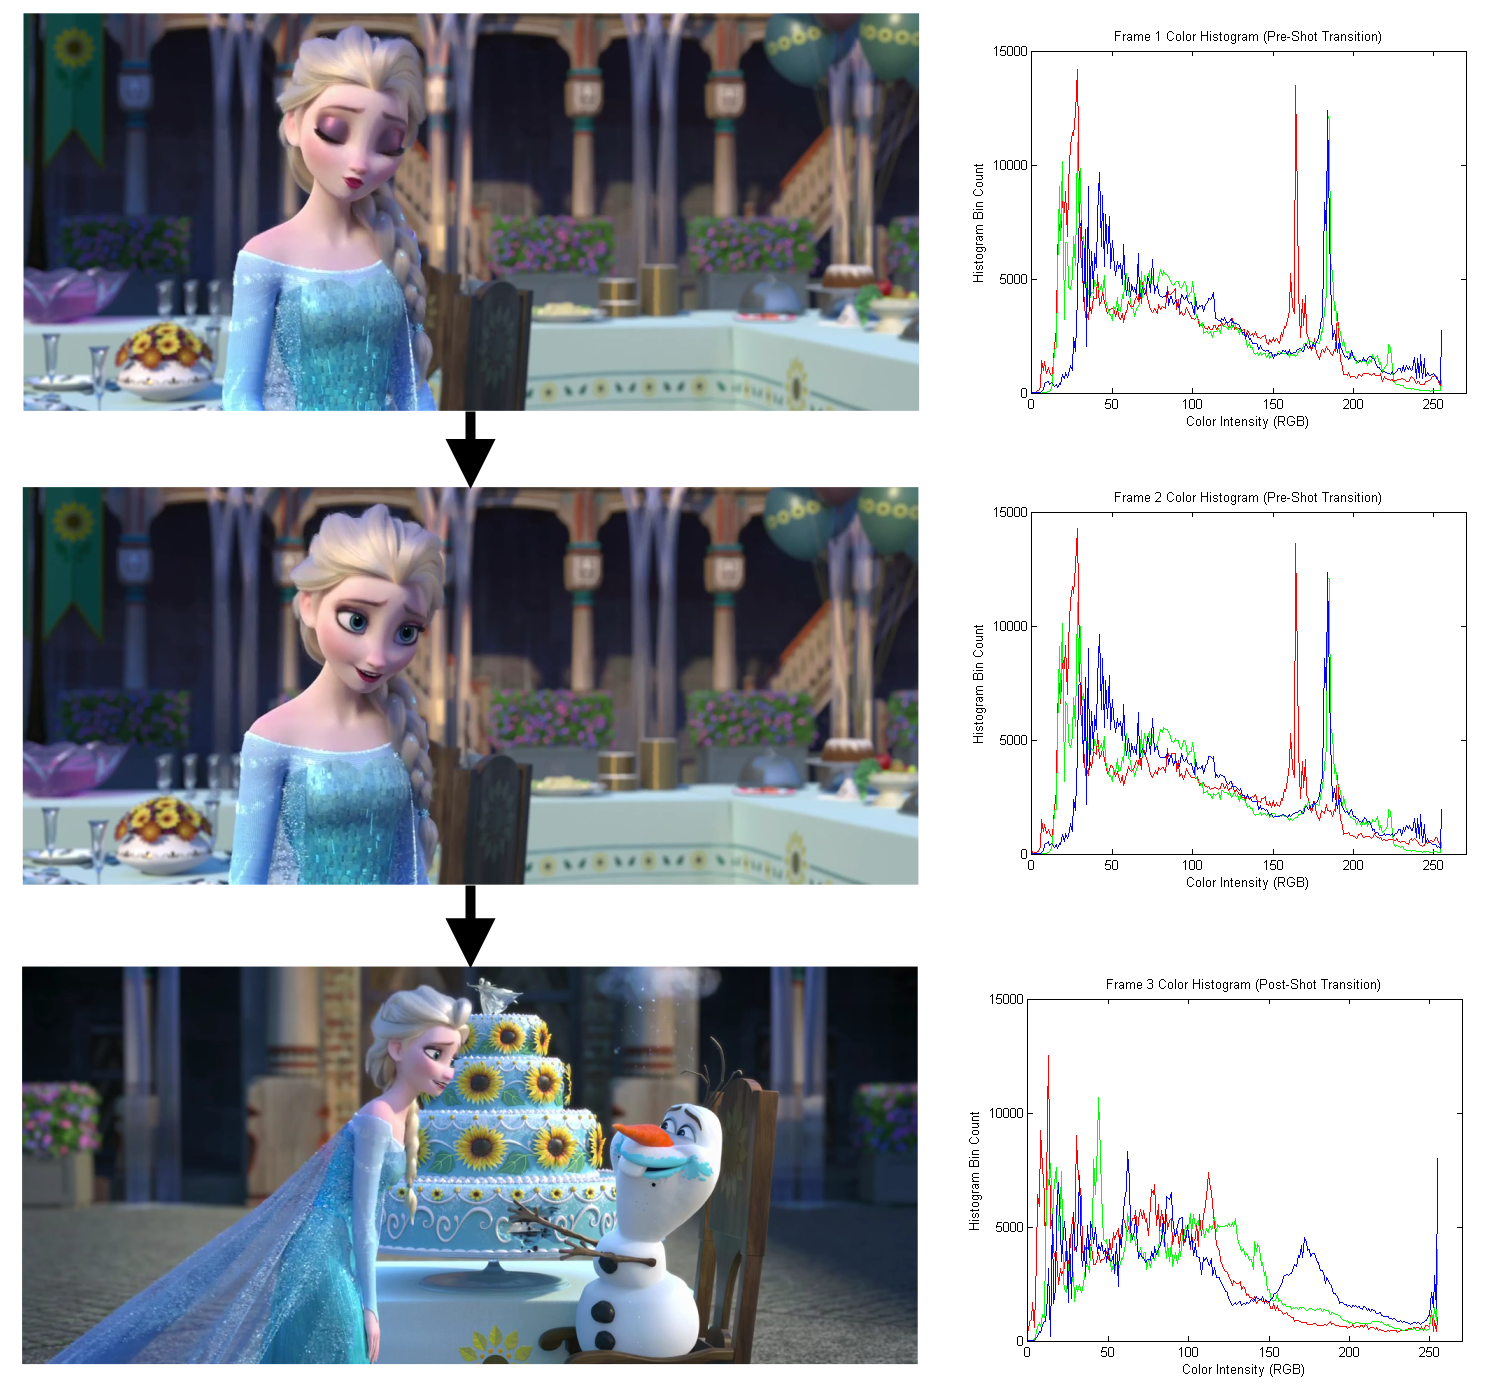
\includegraphics[width=\columnwidth]{histograms_combined.png}
	\caption{Three example video frames are shown on the left, with their color histograms on the right. The first two frames are similar, and are part of the same shot; note their similar histograms. The third frame, only a fraction of a second later, has a starkly different histogram, and would thus be detected as a new shot.}
	\label{f:histograms_combined}
\end{figure}

\subsubsection{Shot Length}
%mean, std dev,min and max
Once the time-stamps of shot transitions were recognized, we were also able to calculate metrics based on the length of shots: mean, standard deviation, and minimum/maximum shot lengths. The mean shot length varied greatly on our sample set, from 0.2 seconds to 3 seconds.

\subsubsection{Detail Score}
%std dev, min and max
We defined a measure of the amount of complex detail in a trailer through the use of the Canny edge detection filter \cite{canny}. By applying the Canny algorithm to a given frame, we can calculate a binary mask wherein all of the ``edge pixels" in that frame have a value of 1. Then, by summing all of pixels in the frame, and summing all of the frames into the trailer, we can get a total ``detail score" for that trailer. That score can then be scaled by the number of frames to normalize and find the average detail per frame. We calculated detail score features (including mean value, standard deviation, and minimum/maximum values) in this way. See Fig.~\ref{f:canny_combined} for an example of edge-detected images from which detail scores were calculated.

\begin{figure}[h]
	\centering
	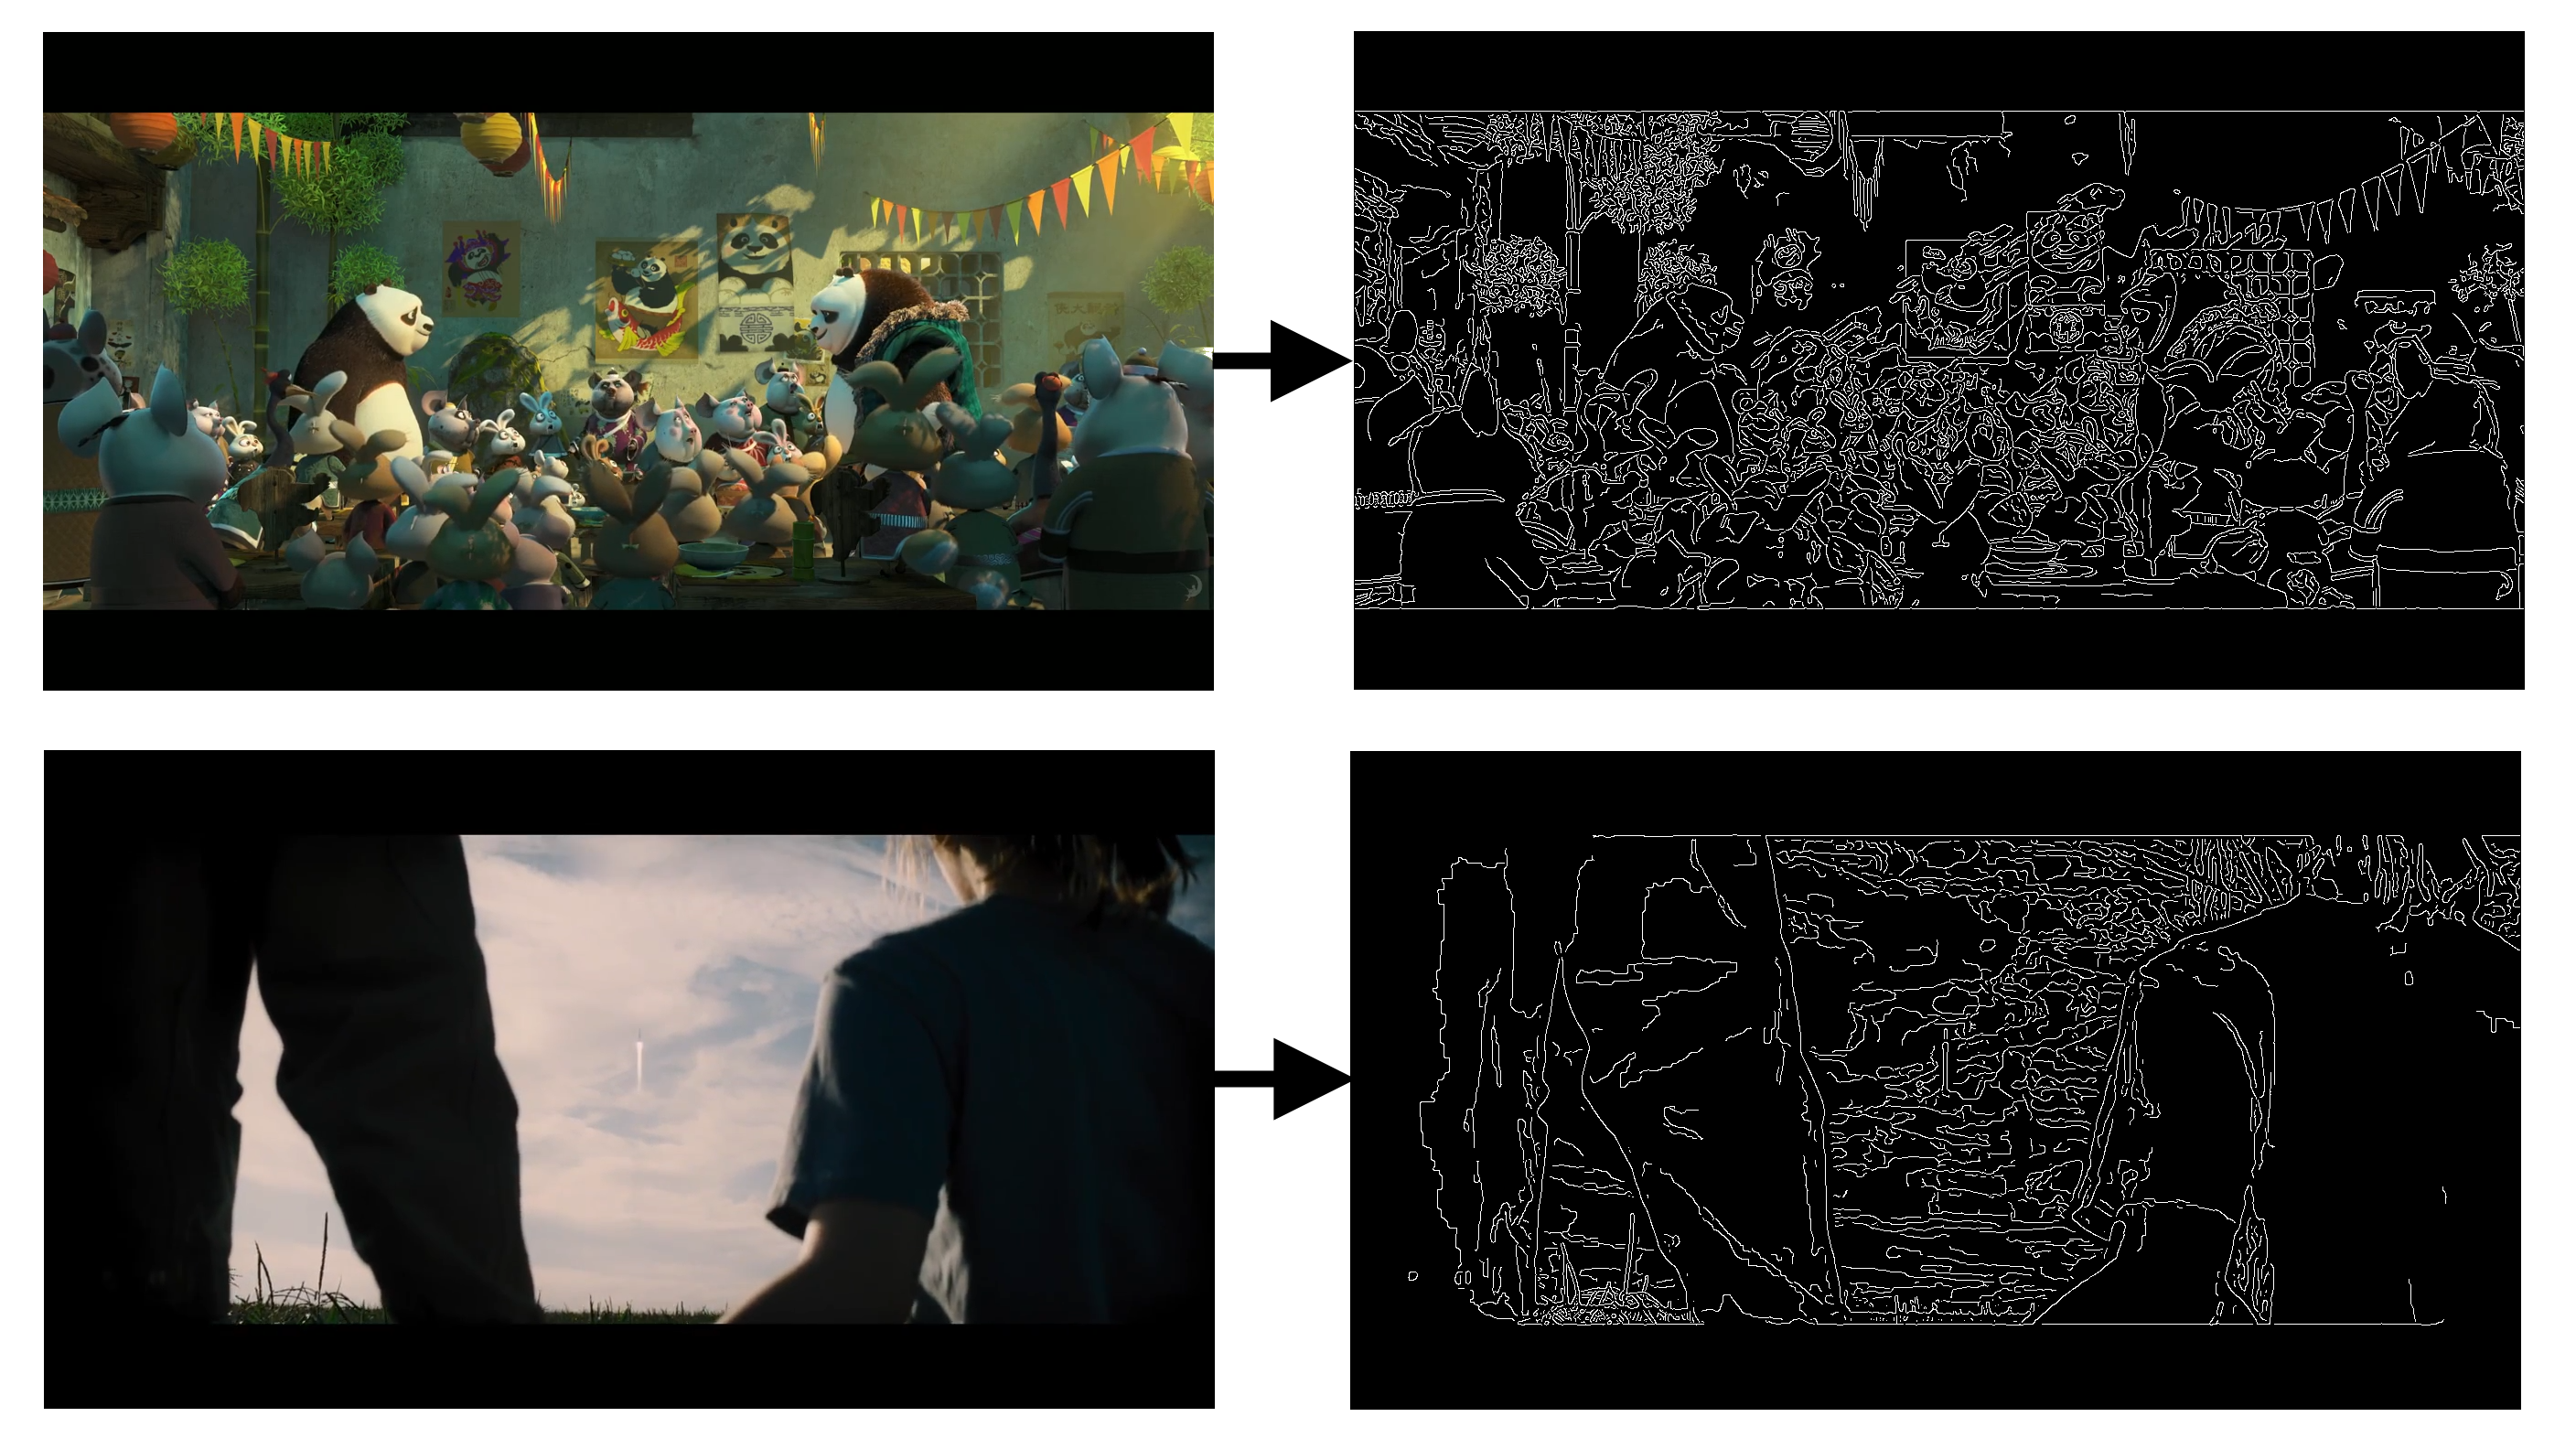
\includegraphics[width=\columnwidth]{canny_combined.png}
	\caption{Two example video frames are shown on the left, with their Canny edge-detected versions on the right. By counting the white (edge) pixels in the images on the right, a ``detail score" can be calculated, as a rough metric of the detail complexity of the frame.}
	\label{f:canny_combined}
\end{figure}

\subsubsection{Dark Scenes}
%count, percentage, mean length, std dev, min and max
We defined the notion of a ``dark scene" as a period of consecutive frames with very low average values (i.e., black transitions). Their lengths were recorded, from which mean length, standard deviation of length, and minimum/maximum lengths were calculated. The percentage of dark scene frames in each trailer was also calculated. 

\subsection{Feature Generation via Audio Processing}
%keyword : FFT, 
From the trailer videos, we isolated the audio component using a sampling frequency of 44.1 kHz. A series of analyses was performed on this audio data in order to extract features.

\subsubsection{Volume}
\textit{Mean}: Mean volume for each trailer was calculated by averaging the amplitudes of sound waves over the entire duration of the trailer. One motivation behind extracting this feature was that a trailer saturated with loud noises would have larger value of mean volume than trailers with relatively calm sounds. Also, typically trailers with loud noises--explosions, jet noise, shouting, etc.--are associated with genres such as action, thriller, and adventure. On the other hand, trailers with calm audio, and even some quietness, may be associated with genres such as drama, history, and family. \\

\textit{Standard Deviation}: all trailers were sourced from a single film site, but there was no guarantee that their audio was all equalized to the similar degree, especially because many were produced by different companies. Thus, a higher mean volume could simply indicate a trailer that's louder in general due to different equalization characteristics, rather than an abundance of loud sound events. In order to get a sense of the variation of volume in each trailer, we calculated standard deviation of the sound wave amplitude over the entire trailer as well.\\

\textit{Minimum and Maximum}: Minimum and maximum volume for each trailer were calculated based on the waveform data. On a scale from 0.0 to 1.0, most trailers had a minimum volume near 0.0, while some had marginally higher minimum values, such as 0.03. Maximum volume generally fell into the range of 0.1 to 0.5.

\subsubsection{Sudden Rise/Fall of Volume}
We defined the concept of a sudden rise and sudden fall of volume. Respectively, these represent an increase and a decrease of volume within a small time period, possessing a magnitude larger than the standard deviation of the volume across the whole trailer. Identifying the number of these events within a trailer's audio allowed us to study its audio dynamics, as we intuited that sudden increases of volume might be common during trailers that sought to startle viewers (such as those horror or action films).

\begin{figure}[h]
	\centering
	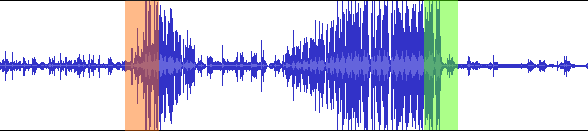
\includegraphics[width=\columnwidth]{audio_peaks.png}
	\caption{An audio sample is shown, with a sudden rise and a sudden fall highlighted in orange and green, respectively. Note that the interior fall and rise are not captured as sudden changes, due to their more gradual change.}
	\label{f:audio_peaks}
\end{figure}


\subsubsection{Percentage of Sound Corresponding to Different Octave Bands}
For this feature, the waveform of each trailer was transformed to the frequency domain using the Fast Fourier transform (FFT). Its frequencies were divided into eleven bands in the audible range, commonly defined as octave bands (11Hz $\sim$ 22720Hz). The magnitudes of the frequency components in each band were summed together, and normalized so that the sum of magnitudes of all octave bands would be 1. The resulting binned magnitudes represented the composition of sounds of each trailer with respect to these eleven octave bands. 

\subsection{Use of Features in Machine Learning Algorithm}
%keyword: binary decision tree
All extracted features from each trailer were compiled into a single comma-separated variable (CSV) spreadsheet. In addition to our generated features, the spreadsheet contained the genre labels for each trailer as well. Movies were not limited to one genre. For instance, there were movie trailers with multiple genre labels such as action-comedy, or mystery-horror-thriller. This spreadsheet was passed on to Matlab's fit binary classification decision tree function (\textit{fitctree}) to build a decision tree. Only 80\% of the trailers randomly selected from the full set of trailers were used for building the tree. This subset is known as a trainer set. The tree was then used to predict the entire range of trailers using Matlab's classification predict function (\text{predict}), and its success and failure rates were recorded. This process was repeated 40 times, each time with a new set of random trainer sets, for the purpose of cross-validation.

%%%%%%%%%%%%%%%%%%%%%%%%%%%%%%%%%%%%%%%%%%%%%%%%%%%%%%%%%%%%%%%%%%%%%%%%%%%%%%%%
\section{RESULTS}

The rate of success of classification by our algorithm for the top ten most common genres in our dataset is shown in Fig.~\ref{f:success_rate_table}. Drama, with a 65\% successful classification, had the lowest success rate of those tested, but the other 9 genres registered consistently over an 80\% success rate.\\

\begin{figure}[h]
	\centering
	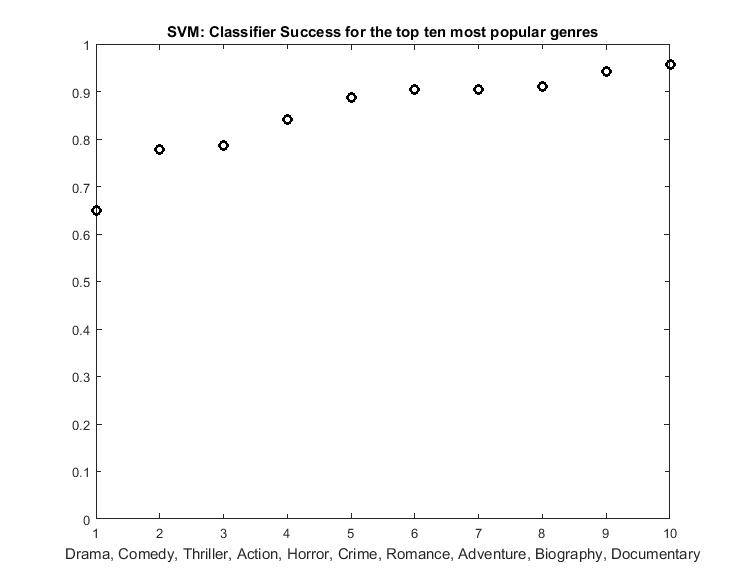
\includegraphics[width=\columnwidth]{success_rate.jpg}
	\caption{Classifier success rate for the ten most common genres.}
	\label{f:success_rate_table}
\end{figure}

In order to gain some insight into what features are important for the classification, we performed a singular value decomposition on the set of movie trailers and their features. As can be seen in the plot of covariances of principal modes (Fig.~\ref{f:mode_covar}), only four modes capture roughly 90\% of the energy.

\begin{figure}[h]
	\centering
	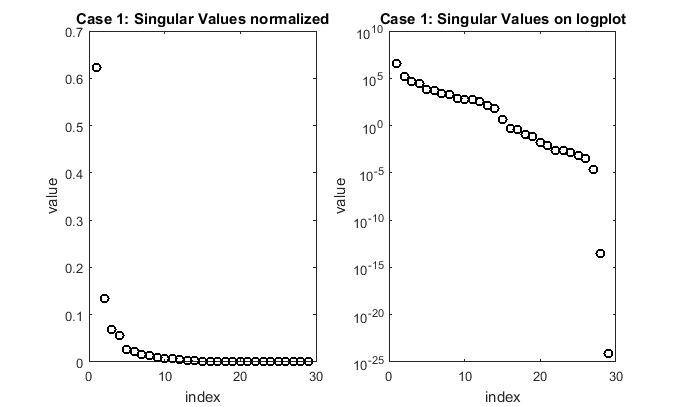
\includegraphics[width=\columnwidth]{mode_covar.jpg}
	\caption{Covariances of each mode.}
	\label{f:mode_covar}
\end{figure}

These four modes consist of features of differing degree. Fig.~\ref{f:mode_composition} displays the weights of each feature in four prominent modes. One can observe that the leftmost ten features are driving factors for these modes. These features are: number of shots, dark scene max. length, total time, average blue color, average green color, average intensity, average red color, dark scene length standard deviation, dark scene mean length and dark scene count. These results suggest that our machine learning algorithm relies mainly on chromatic and luminous qualities of trailers, as eight of the ten most important features describe color and brightness of scenes in trailers. In other words, from the computer's perspective, trailers of different genres sound similar, but some are more colorful than others.

\begin{figure}[h]
	\centering
	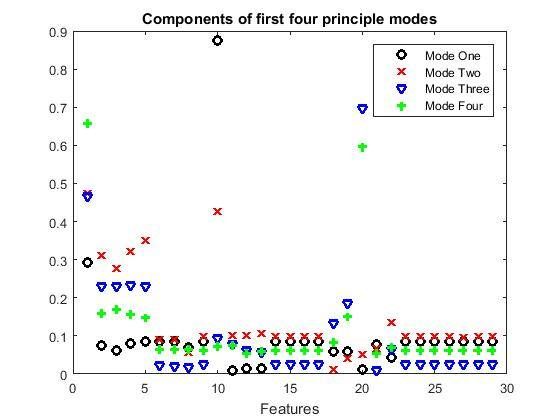
\includegraphics[width=\columnwidth]{mode_comp.jpg}
	\caption{Compositions of features for each mode.}
	\label{f:mode_composition}
\end{figure}

We experimented with the concept of dimensional reduction by trying classification using one, two and four modes. The ratees of success are plotted in Fig.~\ref{f:modal_redx}. Surprisingly, the difference in success rate between one-mode classification and all-mode classification is only about 10\%.
\onecolumn

\begin{figure}
	\centering
	\begin{subfigure}[b]{0.475\textwidth}
		\centering
		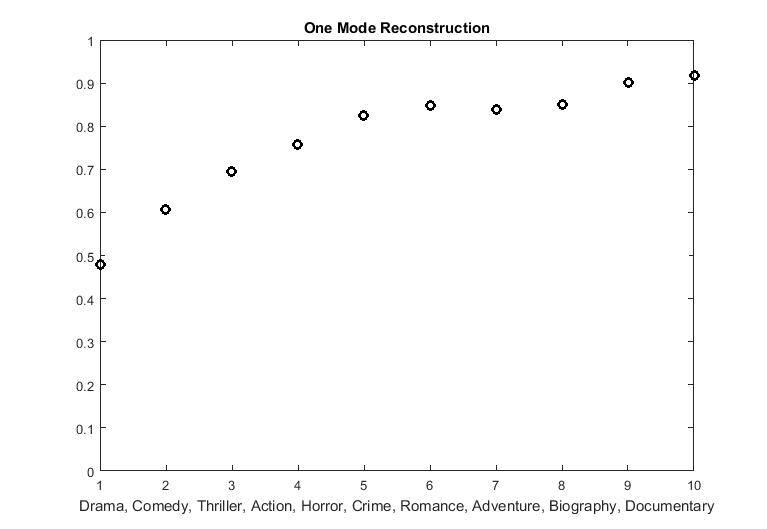
\includegraphics[width=\textwidth]{one_mode_appx}
	\end{subfigure}
	\hfill
	\begin{subfigure}[b]{0.475\textwidth}  
		\centering 
		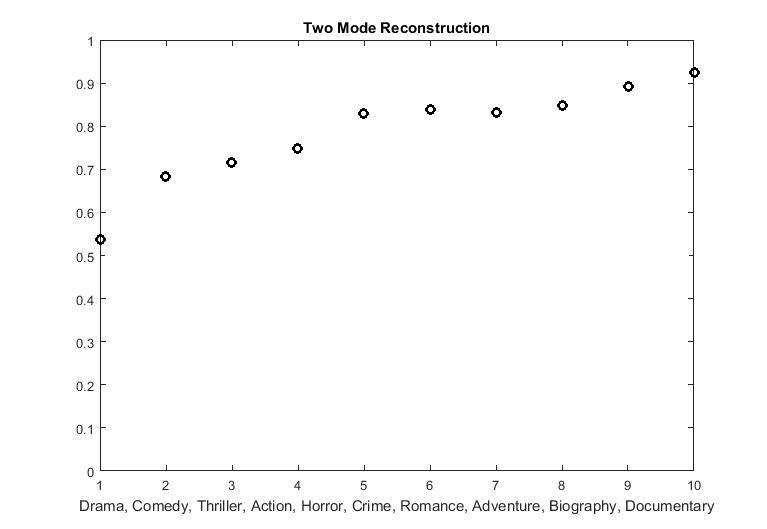
\includegraphics[width=\textwidth]{two_mode_appx}
	\end{subfigure}
	\vskip\baselineskip
	\begin{subfigure}[b]{0.475\textwidth}   
		\centering 
		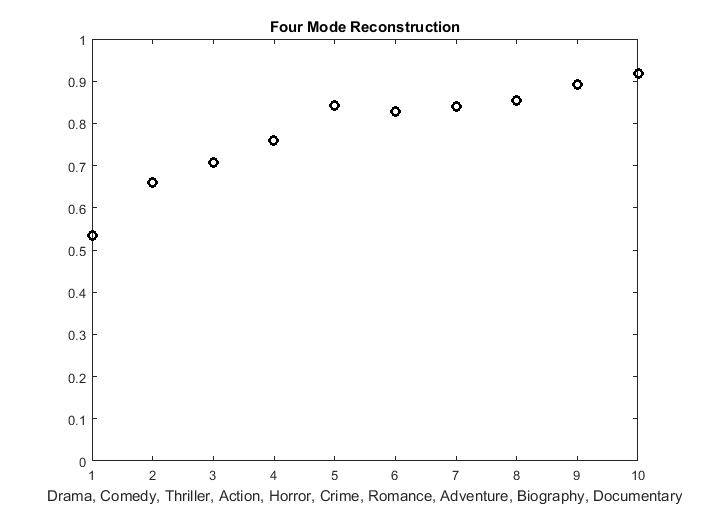
\includegraphics[width=\textwidth]{four_mode_appx}
	\end{subfigure}
	\quad
	\begin{subfigure}[b]{0.475\textwidth}   
		\centering 
		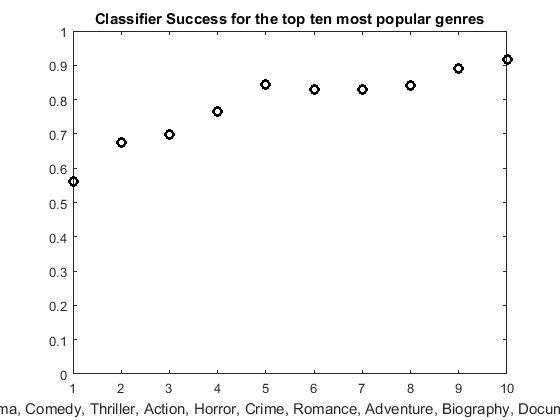
\includegraphics[width=\textwidth]{orig_mode}
	\end{subfigure}
	\caption{Classifications made with one, two and four mode approximations compared to the original classification made with a complete set of modes.}
	\label{f:modal_redx}
\end{figure}

\twocolumn

%%%%%%%%%%%%%%%%%%%%%%%%%%%%%%%%%%%%%%%%%%%%%%%%%%%%%%%%%%%%%%%%%%%%%%%%%%%%%%%%
\section{LESSONS LEARNT}
One failed attempt to acquire features from the audio portion of movie trailers was to perform a Principal Component Analysis (PCA) using singular value decomposition. The goal of this process was to identify a series of principal modes and their components in each of the movie trailers. The hypothesized that the values of principal components could be used as features. We clipped 10-second portion of audio from each trailer to reduce the size of the data. Nonetheless, the matrix at which the singular value decomposition was to be performed had a size of 958-by-227150. This was computationally very expensive, with a runtime on the order of 10+ hours on modern personal computer. Furthermore, there was no guarantee that 10-second clipping would capture a signature sound of each trailer. (In a preliminary attempt, a 10-second clip was clipped at the timestamp of $t=\frac{total\, time}{2}$). Given these reasons, the attempt was deemed implausible in the sense of cost-benefit, and was abandoned.

%%%%%%%%%%%%%%%%%%%%%%%%%%%%%%%%%%%%%%%%%%%%%%%%%%%%%%%%%%%%%%%%%%%%%%%%%%%%%%%%
\section{FUTURE WORK}



%%%%%%%%%%%%%%%%%%%%%%%%%%%%%%%%%%%%%%%%%%%%%%%%%%%%%%%%%%%%%%%%%%%%%%%%%%%%%%%%
\section{CONCLUSION}



%%%%%%%%%%%%%%%%%%%%%%%%%%%%%%%%%%%%%%%%%%%%%%%%%%%%%%%%%%%%%%%%%%%%%%%%%%%%%%%%
\section{ACKNOWLEDGMENTS}

We would like to thank Dr. Nathan Kutz for his advice and feedback on our techniques used in this project. We'd also like to thank Kam Chancellor, because Nathan would want us to.

%%%%%%%%%%%%%%%%%%%%%%%%%%%%%%%%%%%%%%%%%%%%%%%%%%%%%%%%%%%%%%%%%%%%%%%%%%%%%%%%

\begin{thebibliography}{99}
\bibitem{Rasheed}
Rasheed Z., Sheikh Y., Shah M., {\it On the Use of Computable Features for Film Classification}, IEEE Transactions on Circuits and Systems for Video Technology, Vol.15 No.1, Jan. 2005.

\bibitem{cv2}
{\it OpenCV | OpenCV}. Itseez. Web. 09 Mar. 2016. http://opencv.org/.

\bibitem{canny}
Canny, J., {\it A Computational Approach To Edge Detection}, IEEE Trans. Pattern Analysis and Machine Intelligence, 8(6):679–698, 1986.

\end{thebibliography}

\end{document}
